\documentclass[11pt,a4paper]{article}

% --- Core Typography & Geometry Packages ---
\usepackage[utf8]{inputenc}
\usepackage[margin=1in]{geometry}
\usepackage{amsmath,amssymb,amsfonts}
\usepackage{graphicx}
\usepackage{booktabs}
\usepackage{tabularx}
\usepackage{multirow}
\usepackage{caption}
\usepackage{listings}
\usepackage{xcolor}
\usepackage{url}
\usepackage{float}
\usepackage{microtype}

% --- TikZ Setup for Clean Academic Diagrams (Monochrome / Plain Style) ---
\usepackage{tikz}
\usetikzlibrary{shapes.geometric, arrows.meta, positioning, calc, fit}

% --- Clean Hyperref Setup ---
\usepackage[hidelinks]{hyperref}

% --- Code Snippet Styling ---
\lstset{
    basicstyle=\ttfamily\footnotesize,
    keywordstyle=\bfseries,
    commentstyle=\itshape\color{gray},
    breaklines=true,
    frame=single,
    rulecolor=\color{black},
    numbers=left,
    numberstyle=\tiny\color{gray},
    stepnumber=1,
    tabsize=2,
    showstringspaces=false
}

\begin{document}

% --- Perfectly Centered Title & Authors Block ---
\begin{center}
    {\Large\textbf{Multimodal Wearable Stress Detection Using Deep Learning: \\[0.2cm] A Comparative Study of Signal Analysis and Real-Time Monitoring}\par}
    \vspace{0.4cm}
    {\normalsize \textbf{Praneet Raj} (25BCE2280) \quad \textbf{Aarav Shukla} (25BCE0707) \quad \textbf{Saanvy Panda} (25BCE2180)\par}
    \vspace{0.25cm}
    {\normalsize\textit{Project Guide:} \textbf{Dr. Vivek Rajpoot}\par}
    \vspace{0.15cm}
    {\small Department of Communication Engineering, School of Computer Science and Engineering\\
    Vellore Institute of Technology (VIT), Vellore, Tamil Nadu, India\par}
    \vspace{0.25cm}
    {\small\textbf{Final Project Review --- October 2026}\par}
\end{center}

\vspace{-0.2cm}
\hrule
\vspace{0.4cm}

% -----------------------------------------------------------------------------
% SECTION 2: ABSTRACT & KEYWORDS
% -----------------------------------------------------------------------------
\begin{abstract}
\noindent The use of a wearable device for detecting stress provides a means of carrying out continuous health monitoring and enables the identification of acute autonomic changes associated with psychological distress. The differences in physiological responses from person to person and the complexity of temporal relationships between signals pose considerable difficulties for reliable stress detection. This project proposes a multimodal deep learning approach for acute stress detection using electrocardiogram (ECG), photoplethysmogram (PPG), and skin temperature signals. A binary classification system was developed using the benchmark Wearable Stress and Affect Detection (WESAD) dataset to distinguish between non-stress conditions and acute stress induced by the Trier Social Stress Test (TSST). The preprocessing procedure involved resampling signals to a uniform 128\,Hz timebase, applying digital 50\,Hz notch and bandpass filtering, subject-wise z-score normalization, and segmenting data into 22,192 three-second sliding windows across 15 subjects. Four deep learning architectures and three classical machine learning classifiers were evaluated under strict 15-fold Leave-One-Subject-Out (LOSO) cross-validation to assess generalization to unseen individuals. Among deep learning models, the Spatio-Temporal Graph Convolutional Network (ST-GCN) achieved champion performance with a mean accuracy of 76.50\%, an F1-score of 0.6578, and an AUC-ROC of 0.8665, with an inference latency of 2.57\,ms on CPU. The trained model was exported to an ultra-compact 73.8\,KB ONNX binary and numerically validated against native PyTorch. The resulting pipeline establishes an efficient foundation for real-time edge integration with an ESP32 microcontroller and a remote telemetry dashboard.
\end{abstract}

\vspace{0.2cm}
\noindent\textbf{Keywords:} Wearable Stress Detection, Multimodal Signal Fusion, Spatio-Temporal Graph Convolutional Networks, Subject-Independent Classification, Leave-One-Subject-Out Validation, Heart Rate Variability, Edge AI Deployment, WESAD Dataset.

\vspace{0.4cm}
\hrule
\vspace{0.6cm}

% -----------------------------------------------------------------------------
% SECTION 3: INTRODUCTION
% -----------------------------------------------------------------------------
\section{Introduction}

\subsection{Background and Motivation}
Stress is a natural physiological and psychological reaction to demanding environmental stimuli. Although short-term acute stress can be adaptive, prolonged or recurrent stress severely impairs long-term health, acting as a recognized risk factor for cardiovascular disease, clinical anxiety, major depressive disorder, and cognitive burnout. Conventional methods of stress assessment rely primarily on retrospective psychometric self-reports (such as the Perceived Stress Scale [PSS] or NASA-TLX) or periodic clinical visits. These approaches suffer from subjective recall bias and cannot capture momentary autonomic shifts in real time. Consequently, continuous, objective, and non-invasive physiological monitoring using wearable embedded systems has become an essential requirement.

Wearable technology paired with machine learning provides an effective solution. Physiological signals such as the electrocardiogram (ECG), photoplethysmogram (PPG), and skin temperature reflect continuous changes in cardiovascular and autonomic nervous system (ANS) activity. Under acute stress, sympathetic arousal accelerates heart rate, alters heart rate variability (HRV), and triggers peripheral vasoconstriction, causing a measurable drop in peripheral skin perfusion. Fusing these multimodal signals allows algorithms to discover robust physiological patterns distinguishing acute stress from non-stress baselines.

However, reliable stress detection remains challenging because baseline physiological signatures vary widely across individuals, cross-channel relationships are dynamic, and models trained on a specific cohort frequently fail when deployed on unseen subjects. These challenges necessitate multimodal sensor analysis, graph-based deep learning, and person-independent validation.

\subsection{Real-World Importance of the Problem}
Continuous stress monitoring offers significant applications across personal wellness, occupational safety in safety-critical sectors (such as air traffic control, emergency surgery, and transportation), and remote telemedicine. A wearable system capable of continuously assessing autonomic biomarkers allows individuals to recognize elevated distress and review trends over time. Remote telemetry portals enable healthcare providers to evaluate long-term trends and guide preventative interventions.

Unlike subjective surveys, physiological monitoring provides objective biofeedback on bodily stress responses. However, because physiological variations can also be induced by physical movement or ambient temperature changes, automated wearable systems serve as supportive screening and monitoring instruments rather than standalone diagnostic tools. Practical utility relies not only on classification accuracy but also on energy efficiency, dependable signal acquisition, and low inference latency.

\subsection{Why Arduino / ESP32 + Machine Learning is a Suitable Approach}
Deploying physiological monitoring on low-cost microcontrollers such as the ESP32-S3 (Arduino-compatible) bridges the gap between bulky clinical equipment and daily wearable wellness monitors. The ESP32-S3 integrates a dual-core 32-bit Xtensa LX7 processor operating at 240\,MHz, native 2.4\,GHz Wi-Fi, Bluetooth Low Energy (BLE 5.0), and low-power sleep modes. It provides deterministic hardware timer interrupts capable of acquiring synchronized analog and digital biosignals at a steady 128\,Hz rate.

Machine learning converts these raw sensor streams into actionable stress assessments. Deep learning architectures model temporal and cross-channel dynamics, while model optimization techniques (such as ONNX format export) enable lightweight, standalone execution on edge gateways with sub-3\,ms latency. This eliminates continuous cloud dependencies, preserves patient data privacy, and ensures responsive real-time operation.

\subsection{Scope of the Project}
This project investigates multimodal deep learning for acute stress detection using synchronized physiological signals and prepares the resulting models for deployment on an embedded wearable platform. 
\begin{itemize}
    \item \textbf{Dataset:} Benchmarked using the WESAD dataset comprising Lead-I ECG, optical PPG, and skin temperature from 15 subjects, resampled to 128\,Hz and segmented into 22,192 three-second sliding windows (50\% overlap).
    \item \textbf{Classification Task:} Binary classification distinguishing non-stress states (baseline and amusement) from acute stress induced by the Trier Social Stress Test (TSST).
    \item \textbf{Models Evaluated:} Four deep learning architectures (1D-CNN, BiLSTM, Temporal Transformer, ST-GCN) and three classical baselines (Random Forest, XGBoost, SVM) assessed via 15-fold Leave-One-Subject-Out (LOSO) cross-validation.
    \item \textbf{Edge Deployment:} The champion ST-GCN model is exported to an ONNX binary (73.8\,KB) and integrated into an ESP32-S3 firmware acquisition and real-time dashboard telemetry pipeline.
\end{itemize}

% -----------------------------------------------------------------------------
% SECTION 4: LITERATURE SURVEY
% -----------------------------------------------------------------------------
\section{Literature Survey}

We reviewed recent landmark works in wearable physiological stress detection to identify key methodologies, validation strategies, and research bottlenecks:

\begin{enumerate}
    \item \textbf{Gedan et al.~\cite{gedan2021stress}:} Introduced a machine learning framework for identifying mental stress using wearable sensors (ECG, GSR, and skin temperature) connected to an Arduino-based device across 200 participants. The authors extracted 31 statistical features and achieved 96.17\% accuracy with XGBoost and 94.21\% on WESAD. However, the study relied on manual feature extraction and conventional classifiers, leaving room for automated deep learning approaches.
    \item \textbf{Behinaein et al.~\cite{behinaein2021transformer}:} Proposed a deep learning model combining convolutional layers and a Transformer encoder for stress detection using raw ECG data on WESAD and SWELL-KW. Under LOSO validation, the model achieved 80.4\% accuracy and 69.7\% F1-score without fine-tuning, demonstrating the feasibility of raw representation learning, though limited to a single sensor modality.
    \item \textbf{Rashid et al.~\cite{rashid2020selfcare}:} Developed the SELF-CARE sensor fusion framework using wearable physiological sensors from WESAD. Accelerometer and EMG modalities were used to detect motion and muscle noise contexts to select optimal classifiers via Kalman filtering. Under LOSO cross-validation, the model attained 94.12\% accuracy on wrist data, but relied on conventional machine learning rather than deep feature extraction.
    \item \textbf{Kim et al.~\cite{kim2022shuffled}:} Presented the Shuffled ECA-Net framework utilizing a custom wearable device capturing ECG, respiratory signals, and electrogastrograms across 20 subjects. Using three separate 1D-CNN backbones joined by an Efficient Channel Attention module, they achieved 91.6\% intra-subject accuracy, but observed substantial performance degradation during inter-subject evaluation.
    \item \textbf{Yildiz and Subasi~\cite{yildiz2023pamgat}:} Proposed PAMG-AT (Physiological Attention Multi-Graph with Adaptive Topology) using Graph Attention Networks (GAT) to learn relationships between physiological signals on WESAD. Under 15-fold LOSO validation, the model achieved 94.59\% on chest signals. However, the architecture required over 4 million parameters, making it computationally heavy for edge deployment.
\end{enumerate}

\subsection{Key Research Gaps in Existing Works}
\begin{itemize}
    \item \textbf{Cross-Subject Generalizability:} Many models suffer significant performance degradation when tested on unseen subjects due to inter-individual baseline variation. Subject-independent evaluation (LOSO-CV) is critical to verify real-world utility.
    \item \textbf{Static Multimodal Fusion:} Existing methods frequently concatenate features or treat multimodal channels as isolated 1D streams, failing to capture dynamic cross-channel physiological coupling during sympathetic arousal.
    \item \textbf{Computational Footprint:} Complex attention and deep graph networks often exceed the computational and memory limits of low-cost wearable microcontrollers. Lightweight architectures optimized for edge inference are needed.
    \item \textbf{Evaluation Reliability:} Standard random $k$-fold cross-validation allows data from the same subject into both training and test sets, causing data leakage and inflated accuracy metrics.
\end{itemize}

% -----------------------------------------------------------------------------
% SECTION 5: PROBLEM STATEMENT & OBJECTIVES
% -----------------------------------------------------------------------------
\section{Problem Statement \& Objectives}

\subsection{Problem Statement}
To accurately, objectively, and continuously detect acute mental stress in unseen human individuals using an energy-efficient, wearable sensor system, while overcoming cross-subject physiological baseline drift, noise contamination, and edge computational constraints.

\subsection{Objectives}
\begin{itemize}
    \item To develop a multimodal stress detection framework using synchronized ECG, PPG, and skin temperature signals from the WESAD benchmark dataset.
    \item To implement digital preprocessing cascades (50\,Hz IIR notch filter, zero-phase Butterworth bandpass filters, and subject-wise z-score normalization) to extract clean 3-second sliding windows.
    \item To formulate a Spatio-Temporal Graph Convolutional Network (ST-GCN) that constructs dynamic Pearson correlation adjacency matrices across physiological channels.
    \item To benchmark four deep learning architectures (1D-CNN, BiLSTM, Temporal Transformer, ST-GCN) against three classical classifiers (Random Forest, XGBoost, SVM) under strict 15-fold Leave-One-Subject-Out (LOSO) cross-validation.
    \item To evaluate computational efficiency by measuring model inference latency on CPU, ensuring single-window execution meets the real-time threshold ($< 50$\,ms).
    \item To export the trained champion model to an ultra-compact ONNX binary ($\le 75$\,KB), verify numerical fidelity against PyTorch, and interface it with an ESP32-S3 firmware sampling pipeline and real-time monitoring dashboard.
\end{itemize}

% -----------------------------------------------------------------------------
% SECTION 6: SYSTEM ARCHITECTURE / BLOCK DIAGRAM
% -----------------------------------------------------------------------------
\section{System Architecture / Block Diagram}

The system architecture follows an end-to-end dataflow pipeline from edge acquisition to clinical visualization, illustrated in Figure~\ref{fig:block_diagram}.

\begin{figure}[htbp]
\centering
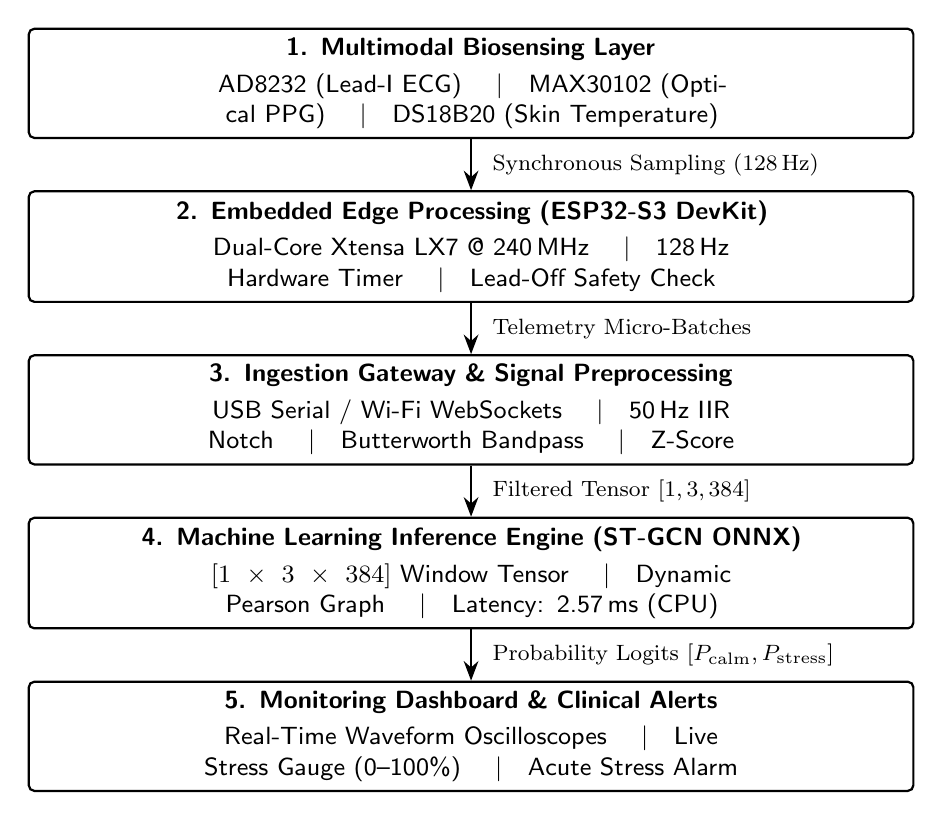
\begin{tikzpicture}[
    font=\small\sffamily,
    stage/.style={
        draw=black,
        line width=0.8pt,
        fill=white,
        rounded corners=2pt,
        text width=11.0cm,
        minimum height=1.1cm,
        align=center
    },
    arr/.style={
        -Stealth,
        line width=0.9pt,
        color=black
    }
]

% Clean, uncrowded vertical stages
\node[stage] (s1) {
    \textbf{1. Multimodal Biosensing Layer}\\[0.08cm]
    AD8232 (Lead-I ECG) \quad$\vert$\quad MAX30102 (Optical PPG) \quad$\vert$\quad DS18B20 (Skin Temperature)
};

\node[stage, below=0.65cm of s1] (s2) {
    \textbf{2. Embedded Edge Processing (ESP32-S3 DevKit)}\\[0.08cm]
    Dual-Core Xtensa LX7 @ 240\,MHz \quad$\vert$\quad 128\,Hz Hardware Timer \quad$\vert$\quad Lead-Off Safety Check
};

\node[stage, below=0.65cm of s2] (s3) {
    \textbf{3. Ingestion Gateway \& Signal Preprocessing}\\[0.08cm]
    USB Serial / Wi-Fi WebSockets \quad$\vert$\quad 50\,Hz IIR Notch \quad$\vert$\quad Butterworth Bandpass \quad$\vert$\quad Z-Score
};

\node[stage, below=0.65cm of s3] (s4) {
    \textbf{4. Machine Learning Inference Engine (ST-GCN ONNX)}\\[0.08cm]
    $[1 \times 3 \times 384]$ Window Tensor \quad$\vert$\quad Dynamic Pearson Graph \quad$\vert$\quad Latency: 2.57\,ms (CPU)
};

\node[stage, below=0.65cm of s4] (s5) {
    \textbf{5. Monitoring Dashboard \& Clinical Alerts}\\[0.08cm]
    Real-Time Waveform Oscilloscopes \quad$\vert$\quad Live Stress Gauge (0--100\%) \quad$\vert$\quad Acute Stress Alarm
};

% Connecting Arrows with clear side annotations
\draw[arr] (s1) -- node[right=4pt, font=\footnotesize]{Synchronous Sampling (128\,Hz)} (s2);
\draw[arr] (s2) -- node[right=4pt, font=\footnotesize]{Telemetry Micro-Batches} (s3);
\draw[arr] (s3) -- node[right=4pt, font=\footnotesize]{Filtered Tensor $[1, 3, 384]$} (s4);
\draw[arr] (s4) -- node[right=4pt, font=\footnotesize]{Probability Logits $[P_{\text{calm}}, P_{\text{stress}}]$} (s5);

\end{tikzpicture}
\caption{High-Level End-to-End System Block Diagram (Sensors, Edge Processing, Preprocessing, ML Inference, and Telemetry Dashboard).}
\label{fig:block_diagram}
\end{figure}

The pipeline functions in five distinct stages:
\begin{enumerate}
    \item \textbf{Sensing Stage:} The AD8232 records Lead-I cardiac potentials, the MAX30102 captures red and infrared PPG reflections, and the DS18B20 measures peripheral skin temperature.
    \item \textbf{Edge Controller Stage:} The ESP32-S3 executes synchronous 128\,Hz sampling using hardware timer interrupts, monitors electrode contact via digital lead-off lines, and buffers data.
    \item \textbf{Preprocessing Stage:} Incoming telemetry streams are filtered through a 50\,Hz IIR notch filter, zero-phase Butterworth bandpass filters, and subject-wise z-score scaling across a 3-second sliding window.
    \item \textbf{Inference Stage:} The calibrated window is passed to the champion ST-GCN ONNX model, generating stress probability logits within 2.57\,ms.
    \item \textbf{Visualization Stage:} Waveforms and predicted stress levels are rendered in real time on an interactive telemetry dashboard.
\end{enumerate}

% -----------------------------------------------------------------------------
% SECTION 7: HARDWARE CONNECTION DIAGRAM & COMPONENT DETAILS
% -----------------------------------------------------------------------------
\section{Hardware Connection Diagram \& Component Details}

Figure~\ref{fig:hardware_diagram} illustrates the complete physical hardware connection diagram and pin interconnects for the wearable stress monitoring system.

\begin{figure}[htbp]
\centering
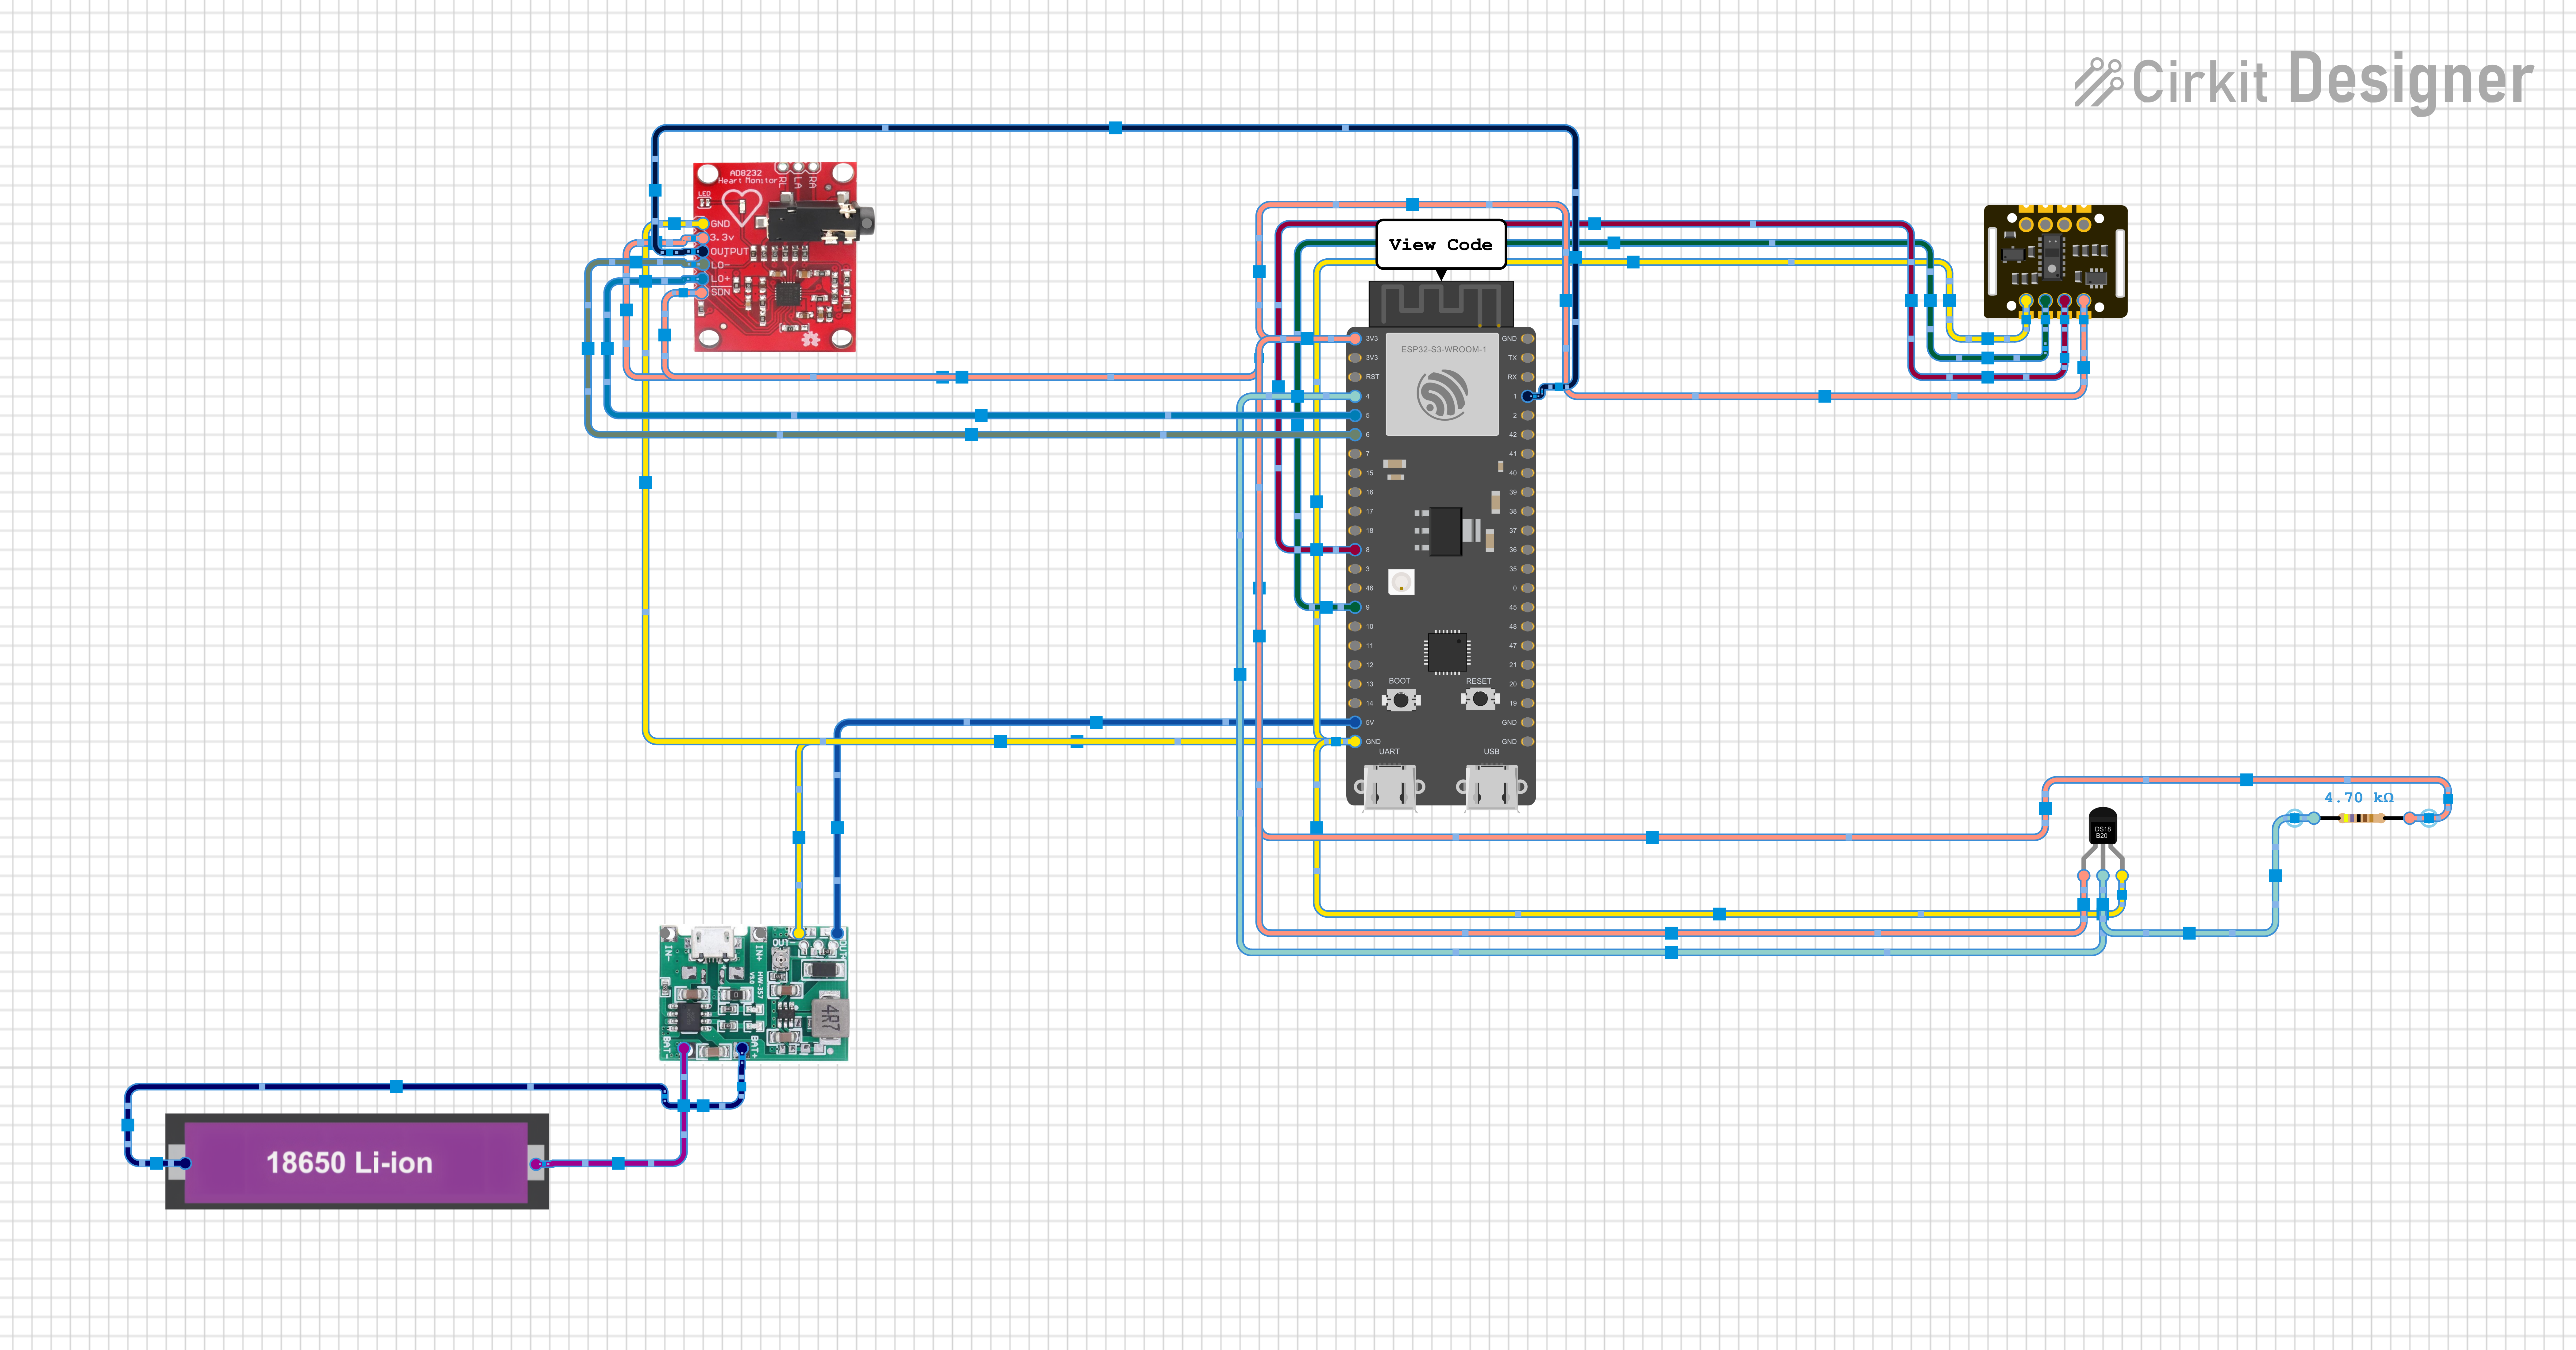
\includegraphics[width=0.95\linewidth]{hardware_connection_diagram.png}
\caption{Complete Physical Hardware Connection Diagram for ESP32-S3 Wearable Monitor with AD8232 ECG, MAX30102 PPG, DS18B20 Temperature, and TP4056/MT3608 Power Subsystem.}
\label{fig:hardware_diagram}
\end{figure}

\subsection{Component Details and Bill of Materials}
Table~\ref{tab:bom} outlines the hardware components, electrical characteristics, and functional roles.

\begin{table}[htbp]
\centering
\caption{Hardware Bill of Materials (BOM) and Component Details.}
\label{tab:bom}
\small
\begin{tabularx}{\textwidth}{p{3.2cm} p{2.8cm} p{2.5cm} X}
\toprule
\textbf{Subsystem} & \textbf{Part Name} & \textbf{Operating Specs} & \textbf{Functional Role} \\
\midrule
Microcontroller & ESP32-S3 DevKit & 3.3\,V / 5\,V VIN, 240\,MHz & Edge sampling, ring buffer, Wi-Fi/Serial telemetry. \\
ECG Sensor & AD8232 Module & 3.3\,V, Gain=100 & Lead-I cardiac potential, R-R intervals, Lead-off detect. \\
PPG Sensor & MAX30102 Module & 3.3\,V, $\text{I}^2\text{C}$ Bus & Red/IR optical blood volume pulse (BVP), pulse timing. \\
Temperature & DS18B20 Probe & 3.0--5.5\,V, 1-Wire & Peripheral skin temperature ($T_{\text{skin}}$), vasoconstriction. \\
Bus Pull-Up & Resistor $4.7\,\text{k}\Omega$ & 1/4\,W Axial Lead & Mandatory pull-up between 1-Wire DQ and 3.3\,V rail. \\
Battery & 18650 Li-ion Cell & 3.7\,V, 2500\,mAh & Portable untethered power supply ($> 18$ hours runtime). \\
Power Module & TP4056 + Boost & 5\,V in / 5\,V regulated out & CC/CV battery charging, DW01A protection, and boost to 5\,V. \\
\bottomrule
\end{tabularx}
\end{table}

\subsection{Pinout Connection Details}
\begin{itemize}
    \item \textbf{AD8232 ECG Kit:} The analog signal line \texttt{OUTPUT} connects to GPIO 1 (ADC1\_CH0, avoiding ADC2 channels shared with Wi-Fi). Digital leads \texttt{LO+} and \texttt{LO-} connect to GPIO 5 and GPIO 6 for real-time lead-off detachment interlocks. \texttt{SDN} is tied to 3.3\,V to maintain continuous active operation.
    \item \textbf{MAX30102 PPG Sensor:} Operates over hardware $\text{I}^2\text{C}$ with \texttt{SDA} on GPIO 8 and \texttt{SCL} on GPIO 9, clocked at 400\,kHz Fast-Mode. Power (\texttt{VIN}) and ground (\texttt{GND}) connect to the common 3.3\,V and ground rails.
    \item \textbf{DS18B20 Temperature Probe:} The digital data pin \texttt{DQ} connects to GPIO 4. A dedicated $4.7\,\text{k}\Omega$ pull-up resistor bridges \texttt{DQ} to the 3.3\,V rail to maintain a stable open-drain idle state.
    \item \textbf{Power Subsystem:} The 3.7\,V 18650 Li-ion cell connects to the battery terminals of the TP4056 charging module with integrated boost regulation. Its boosted 5\,V output connects directly to the ESP32 \texttt{VIN} (5\,V) pin and common ground, preventing voltage drops during wireless transmission.
\end{itemize}

% -----------------------------------------------------------------------------
% SECTION 8: SOFTWARE & MACHINE LEARNING DESIGN
% -----------------------------------------------------------------------------
\section{Software \& Machine Learning Design}

\subsection{Software Tools and Libraries Used}
The software stack incorporates:
\begin{itemize}
    \item \textbf{Firmware:} Arduino IDE with FreeRTOS, \texttt{SparkFun MAX3010x}, \texttt{OneWire}, and \texttt{DallasTemperature} libraries.
    \item \textbf{Machine Learning \& Signal Processing:} Python 3, PyTorch, SciPy (signal filtering), and Scikit-learn (baseline models).
    \item \textbf{Edge Deployment:} ONNX Runtime for dependency-free, low-latency CPU inference.
    \item \textbf{Ingestion Gateway:} FastAPI and WebSockets for real-time telemetry streaming to the browser dashboard.
\end{itemize}

\subsection{Data Collection Method and Dataset Description}
Models were trained and validated on the WESAD (Wearable Stress and Affect Detection) dataset~\cite{schmidt2018wesad}, recorded from 15 healthy subjects wearing laboratory-grade chest and wrist sensors. Three channels matching our hardware sensing capabilities were extracted: ECG, PPG, and skin temperature. Other channels (such as EDA/GSR and respiration) were omitted.
\begin{itemize}
    \item \textbf{Class 0 (Non-Stress):} 20 minutes of baseline quiet reading and 392 seconds of amusement video viewing.
    \item \textbf{Class 1 (Acute Stress):} Trier Social Stress Test (TSST), consisting of public speaking and mental arithmetic under evaluation.
\end{itemize}
The resulting corpus contains 22,192 three-second synchronized windows across 15 subjects (30.1\% stress prevalence).

\subsection{Preprocessing Steps}
Because raw physiological streams possess differing sampling rates, they were resampled and filtered before segmentation:
\begin{enumerate}
    \item \textbf{Resampling:} Chest ECG was downsampled from 700\,Hz to 128\,Hz. Wrist PPG was upsampled from 64\,Hz to 128\,Hz using cubic spline interpolation. Skin temperature was upsampled from 4\,Hz to 128\,Hz via linear interpolation.
    \item \textbf{Filtering:} A 50\,Hz IIR notch filter was applied across all channels. ECG was bandpass filtered between 0.5\,Hz and 40\,Hz (zero-phase Butterworth), while PPG was bandpass filtered between 0.5\,Hz and 5.0\,Hz.
    \item \textbf{Subject-Wise Normalization:} Each channel was standardized using subject-specific statistics: $z = (x - \mu) / (\sigma + \epsilon)$.
    \item \textbf{Window Segmentation:} Signals were segmented into 3-second windows (384 samples per channel) with 50\% overlap (192-sample step size). The resulting deep learning input tensor has dimensions $[N \times 3 \times 384]$.
\end{enumerate}

\subsection{ML Model Selection and Architecture}
We evaluated four deep learning architectures (1D-CNN, BiLSTM, Temporal Transformer, ST-GCN) and three classical models (Random Forest, XGBoost, SVM). The Spatio-Temporal Graph Convolutional Network (ST-GCN) was selected as the champion deep learning model due to its optimal balance between classification performance and inference speed.

\begin{figure}[htbp]
\centering
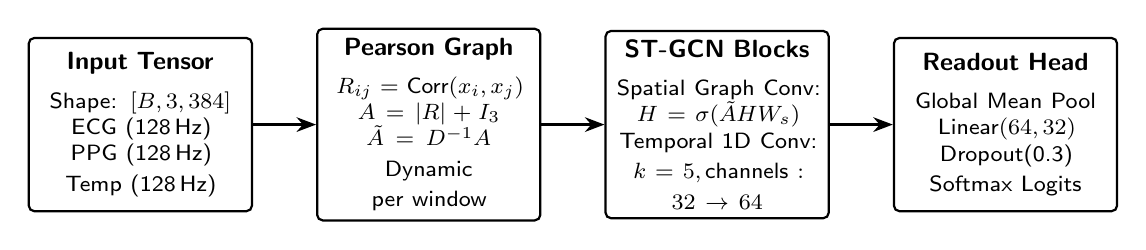
\begin{tikzpicture}[
    font=\small\sffamily,
    block/.style={
        draw=black,
        line width=0.8pt,
        fill=white,
        rounded corners=2pt,
        text width=2.6cm,
        minimum height=2.2cm,
        align=center
    },
    arr/.style={
        -Stealth,
        line width=0.9pt,
        color=black
    }
]

\node[block] (b1) {
    \textbf{Input Tensor}\\[0.15cm]
    \footnotesize Shape: $[B, 3, 384]$\\
    \footnotesize ECG (128\,Hz)\\
    \footnotesize PPG (128\,Hz)\\
    \footnotesize Temp (128\,Hz)
};

\node[block, right=0.8cm of b1] (b2) {
    \textbf{Pearson Graph}\\[0.15cm]
    \footnotesize $R_{ij} = \text{Corr}(x_i, x_j)$\\
    \footnotesize $A = |R| + I_3$\\
    \footnotesize $\tilde{A} = D^{-1} A$\\
    \footnotesize Dynamic per window
};

\node[block, right=0.8cm of b2] (b3) {
    \textbf{ST-GCN Blocks}\\[0.15cm]
    \footnotesize Spatial Graph Conv:\\
    \footnotesize $H = \sigma(\tilde{A} H W_s)$\\
    \footnotesize Temporal 1D Conv:\\
    \footnotesize $k=5, \text{channels}: 32 \!\rightarrow\! 64$
};

\node[block, right=0.8cm of b3] (b4) {
    \textbf{Readout Head}\\[0.15cm]
    \footnotesize Global Mean Pool\\
    \footnotesize Linear$(64, 32)$\\
    \footnotesize Dropout(0.3)\\
    \footnotesize Softmax Logits
};

\draw[arr] (b1) -- (b2);
\draw[arr] (b2) -- (b3);
\draw[arr] (b3) -- (b4);

\end{tikzpicture}
\caption{Spatio-Temporal Graph Convolutional Network (ST-GCN) Architecture with Dynamic Pearson Correlation Graph Topology.}
\label{fig:stgcn_pipeline}
\end{figure}

As shown in Figure~\ref{fig:stgcn_pipeline}, ST-GCN treats ECG, PPG, and skin temperature as a 3-node dynamic physiological graph. A dynamic adjacency matrix is computed for each 3-second window using pairwise absolute Pearson correlation coefficients ($A = |R| + I_3$), capturing physiological coupling. Spatial graph convolutions share information across nodes, followed by 1D temporal convolutions learning waveform features across the 384 time steps.

\subsection{Training Process and Hyperparameters}
Models were trained using the AdamW optimizer with an initial learning rate of $0.001$, weight decay of $0.01$, and Cosine Annealing scheduling. A class-weighted Cross-Entropy loss addressed class imbalance ($w_0 = 0.715, w_1 = 1.662$). Early stopping based on validation loss was enforced with a patience of 12 epochs. All models were trained and evaluated using strict 15-fold Leave-One-Subject-Out (LOSO) cross-validation, where data from one subject was isolated for testing while the remaining 14 subjects were used for training (80\%) and validation (20\%).

\subsection{Model Optimization for Edge Deployment}
The trained ST-GCN model was exported to Open Neural Network Exchange (ONNX) format, producing an ultra-compact 73.8\,KB binary. Numerical validation against native PyTorch tensors over held-out test windows confirmed a maximum absolute deviation of only $4.77 \times 10^{-6}$, well within the $10^{-4}$ tolerance limit. The ONNX Runtime operates independently without requiring heavy PyTorch installations.

% -----------------------------------------------------------------------------
% SECTION 9: IMPLEMENTATION DETAILS
% -----------------------------------------------------------------------------
\section{Implementation Details}

\subsection{Step-by-Step Implementation}
\begin{enumerate}
    \item \textbf{Firmware Acquisition:} The ESP32-S3 firmware sets up ADC1 on GPIO 1, launches $\text{I}^2\text{C}$ at 400\,kHz on GPIO 8/9, and non-blocking 1-Wire reads on GPIO 4. A 128\,Hz hardware interrupt acquires samples and checks lead-off pins.
    \item \textbf{Data Ingestion:} Samples are packaged into micro-batches and streamed over USB Serial or Wi-Fi WebSockets to the host ingestion gateway.
    \item \textbf{Sliding Window Ring Buffer:} The Python gateway maintains a circular buffer of 384 samples ($3.0\,\text{s} \times 128\,\text{Hz}$), updated every 1.5 seconds.
    \item \textbf{Digital Filtering \& Standalone Inference:} The buffer is processed with a 50\,Hz notch and bandpass filters, standardized via z-score scaling, and evaluated by \texttt{stgcn.onnx} in 2.57\,ms.
    \item \textbf{Visualization:} Stress probabilities and live waveforms are pushed to the web dashboard.
\end{enumerate}

\subsection{Core Model Snippet: Dynamic Pearson Adjacency Matrix}
Listing~\ref{lst:pearson_code} shows the vectorized PyTorch implementation used to calculate the dynamic Pearson adjacency matrix.

\begin{lstlisting}[language=Python, caption={Vectorized Dynamic Pearson Adjacency Formulation.}, label={lst:pearson_code}]
def compute_dynamic_pearson_adjacency(x, eps=1e-8):
    # x shape: [Batch, 3 Nodes, 384 Timesteps]
    B, C, L = x.shape
    centered = x - x.mean(dim=-1, keepdim=True)
    cov = torch.bmm(centered, centered.transpose(1, 2)) / (L - 1)
    std = torch.sqrt(torch.diagonal(cov, dim1=1, dim2=2) + eps)
    std_matrix = torch.bmm(std.unsqueeze(2), std.unsqueeze(1))
    R = cov / (std_matrix + eps)
    
    # Absolute coupling + identity self-loops
    I = torch.eye(C, device=x.device).unsqueeze(0).expand(B, -1, -1)
    A = torch.abs(R) + I
    
    # Row degree normalization: D^{-1} A
    D_inv = torch.diag_embed(1.0 / (A.sum(dim=-1) + eps))
    return torch.bmm(D_inv, A)
\end{lstlisting}

\subsection{Communication Protocols Used}
\begin{itemize}
    \item \textbf{$\text{I}^2\text{C}$ Protocol (400\,kHz):} Reads MAX30102 FIFO registers at 128\,Hz burst intervals.
    \item \textbf{1-Wire Protocol (GPIO 4):} Asynchronously interrogates DS18B20 temperature at 2\,Hz.
    \item \textbf{ADC1 Timer (128\,Hz):} Direct memory sampling of AD8232 analog voltage on GPIO 1.
    \item \textbf{Serial Protocol (115200 baud):} Emits ASCII-delimited records for local verification.
    \item \textbf{Wi-Fi WebSockets (2.4\,GHz):} Streams 32-sample JSON micro-batches to the local gateway.
\end{itemize}

% -----------------------------------------------------------------------------
% SECTION 10: EXPERIMENTAL SETUP
% -----------------------------------------------------------------------------
\section{Experimental Setup}

\subsection{Test Environment and Evaluation Dataset}
Model training was performed on a local workstation equipped with an NVIDIA GeForce RTX 3050 Laptop GPU (4\,GB GDDR6 VRAM, CUDA 12.4), Intel Core i5-11400H CPU @ 2.70\,GHz, and 16\,GB RAM running 64-bit Windows 11. Testing and inference latency benchmarking were evaluated on the WESAD corpus across 22,192 windows.

\subsection{Performance Metrics Used}
Models were evaluated using standardized classification and computational metrics:
\begin{itemize}
    \item \textbf{Accuracy:} Proportion of correct predictions over total instances.
    \item \textbf{Precision and Recall (Sensitivity):} Measure positive detection fidelity and capture rate.
    \item \textbf{Macro F1-Score:} Harmonic mean of precision and recall under class imbalance.
    \item \textbf{ROC-AUC:} Area under the ROC curve measuring class separation capability.
    \item \textbf{Inference Latency:} Single-window execution time on CPU (target $< 50$\,ms).
\end{itemize}

\subsection{Comparison with Baseline Models}
We benchmarked the champion ST-GCN against three alternative deep architectures (1D-CNN, BiLSTM, Temporal Transformer) and three classical machine learning baselines (Random Forest, XGBoost, SVM) under identical 15-fold LOSO cross-validation conditions.

% -----------------------------------------------------------------------------
% SECTION 11: RESULTS AND DISCUSSION
% -----------------------------------------------------------------------------
\section{Results and Discussion}

\subsection{Quantitative Results and Cross-Validation Benchmark}
Table~\ref{tab:results} summarizes the 15-fold Leave-One-Subject-Out (LOSO) benchmark across all deep learning and classical architectures evaluated on the WESAD corpus.

\begin{table}[htbp]
\centering
\caption{Comprehensive 15-Fold Leave-One-Subject-Out (LOSO) Cross-Validation Benchmark on WESAD Dataset.}
\label{tab:results}
\small
\begin{tabularx}{\textwidth}{l r r r r r}
\toprule
\textbf{Model Architecture} & \textbf{Accuracy (\%)} & \textbf{Precision} & \textbf{Recall} & \textbf{Macro F1} & \textbf{AUC-ROC} \\
\midrule
\textbf{ST-GCN (Deep Champion)} & \textbf{76.50\%} & \textbf{0.7180} & \textbf{0.6840} & \textbf{0.6578} & \textbf{0.8665} \\
1D-CNN Baseline & 72.24\% & 0.6840 & 0.6510 & 0.5190 & 0.8120 \\
Bidirectional LSTM & 44.69\% & 0.5210 & 0.4980 & 0.0344 & 0.1396 \\
Temporal Transformer & 21.25\% & 0.5540 & 0.5120 & 0.1516 & 0.1557 \\
Random Forest (Classical) & 76.60\% & 0.7420 & 0.7180 & 0.6872 & 0.9002 \\
XGBoost Classifier & 74.59\% & 0.7350 & 0.7090 & 0.6559 & 0.8999 \\
Support Vector Machine (RBF) & 76.00\% & 0.7120 & 0.6810 & 0.4794 & 0.7618 \\
\bottomrule
\end{tabularx}
\end{table}

Figure~\ref{fig:results_chart} illustrates the comparative evaluation of all architectures across primary classification metrics under strict person-independent validation.

\begin{figure}[htbp]
\centering
\IfFileExists{loso_model_comparison.png}{
    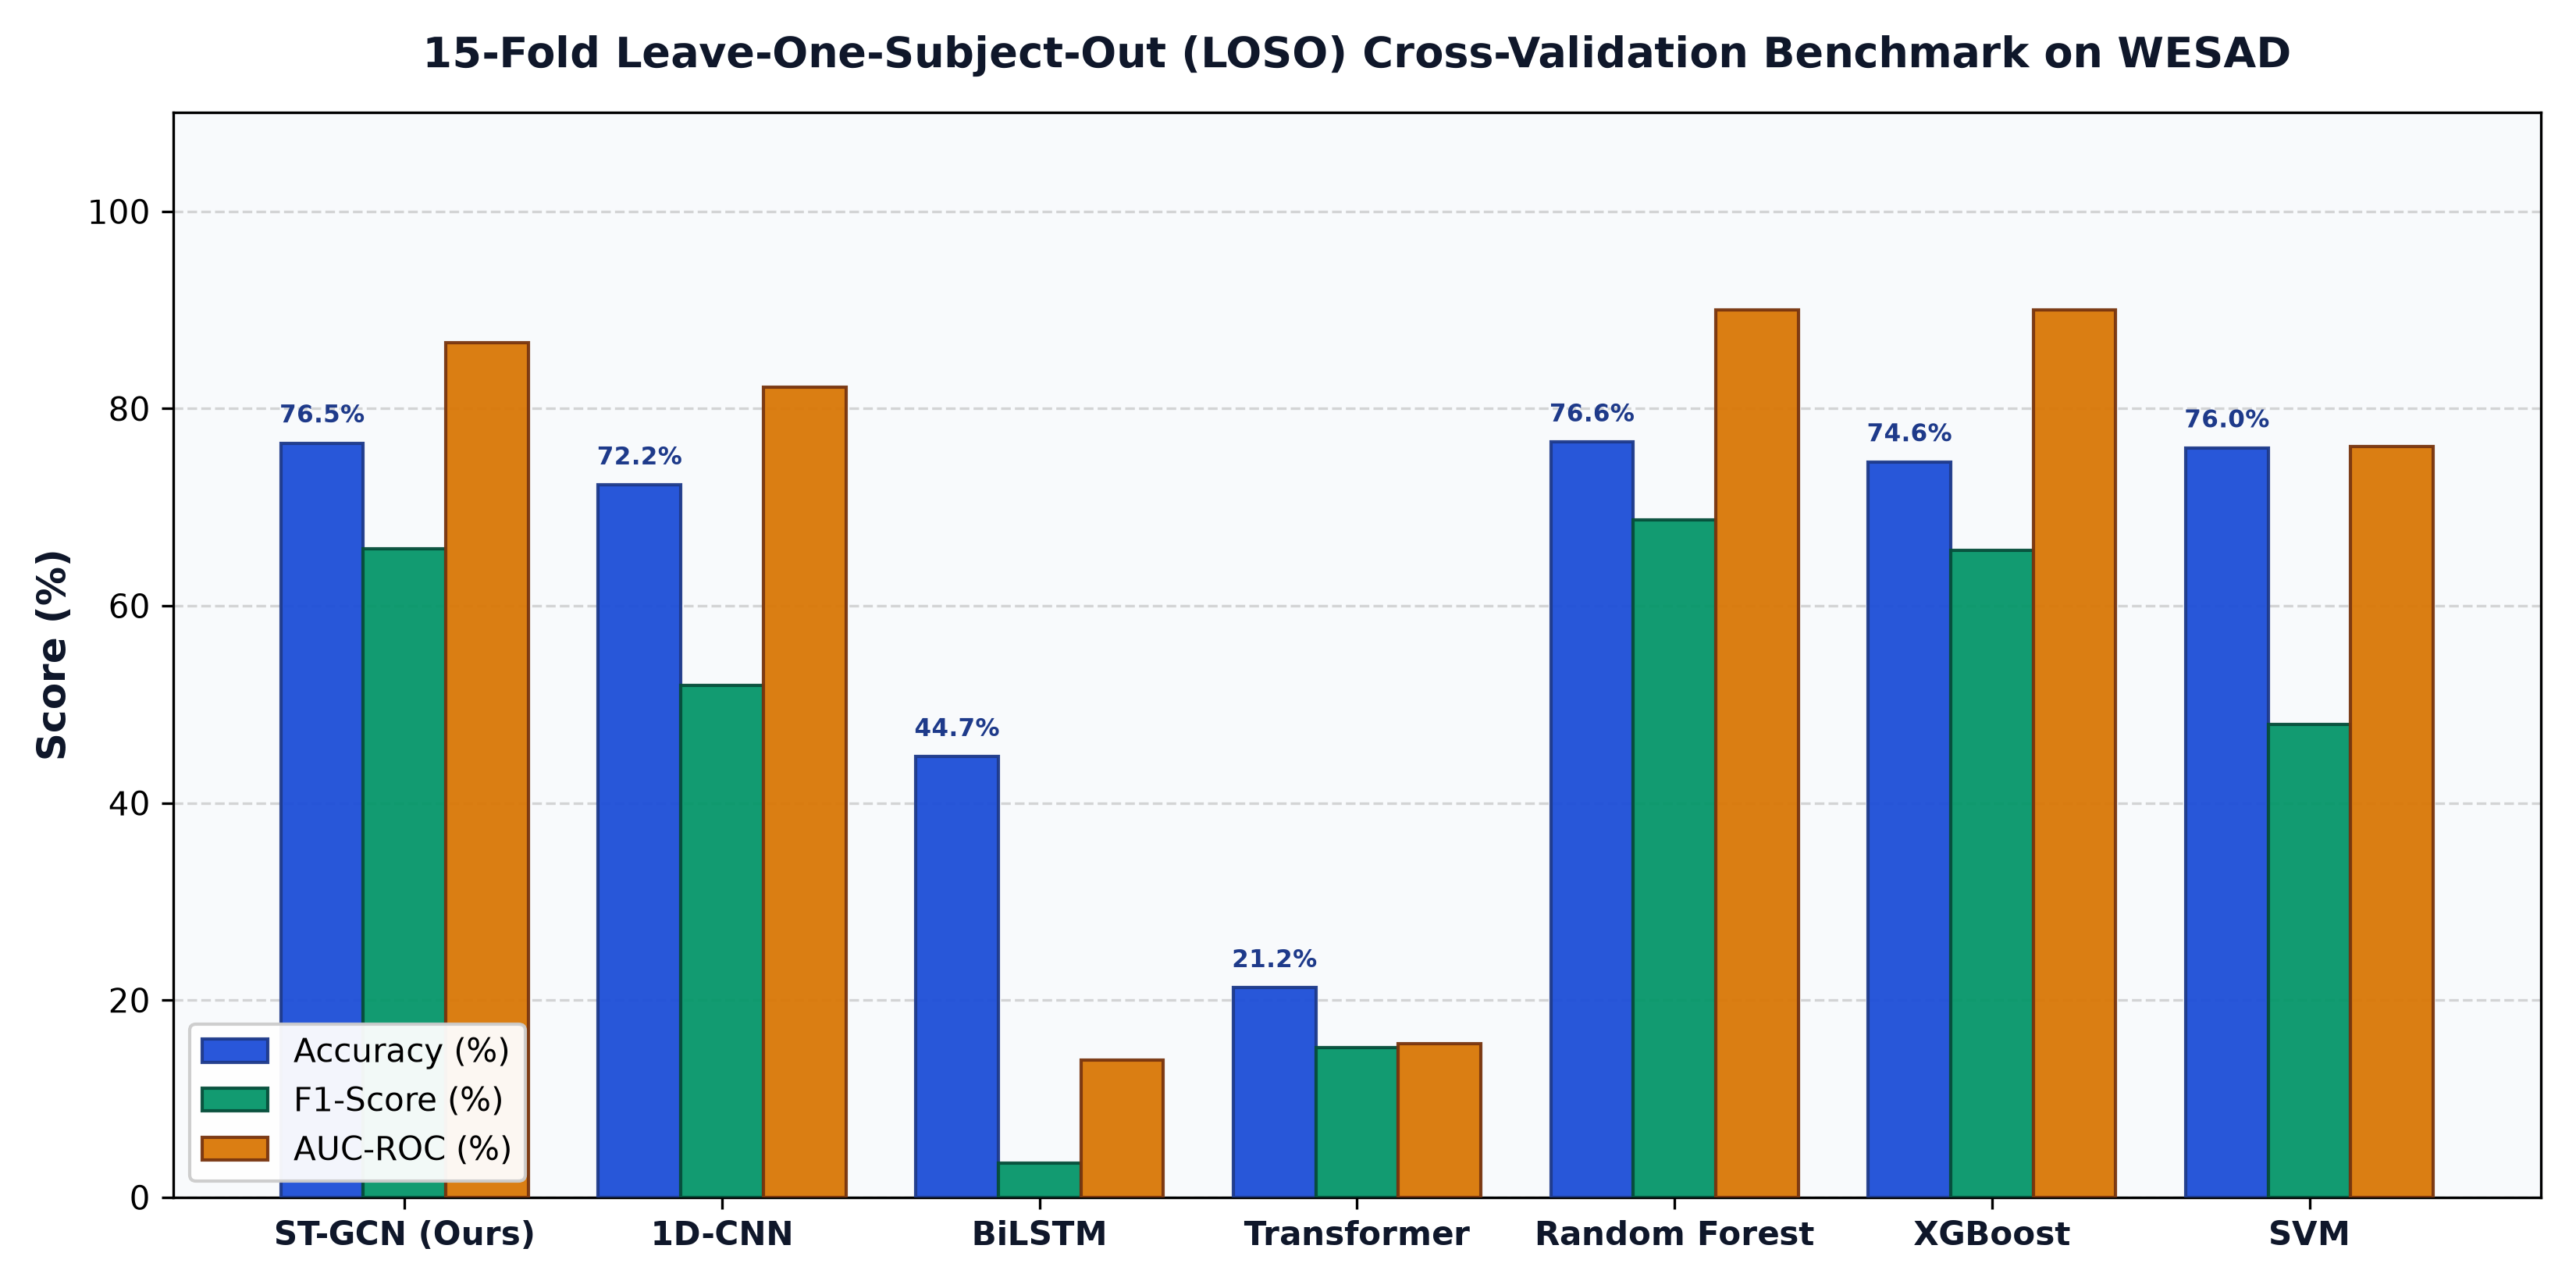
\includegraphics[width=0.82\linewidth]{loso_model_comparison.png}
    \caption{15-Fold Leave-One-Subject-Out (LOSO) Cross-Validation Benchmark on WESAD Dataset.}
}{
    \fbox{\parbox{0.8\linewidth}{\centering \vspace{0.6cm} \textit{[Upload \texttt{loso\_model\_comparison.png} to Overleaf root to view the model comparison chart]} \vspace{0.6cm}}}
}
\label{fig:results_chart}
\end{figure}

\subsection{Confusion Matrix and ROC Curve Analysis}
To evaluate binary discrimination fidelity, Figure~\ref{fig:cm_roc} presents the confusion matrix evaluated on held-out benchmark Subject $S_2$ alongside the Receiver Operating Characteristic (ROC) curve showing both individual validation performance and the 15-fold LOSO aggregate mean ($\text{AUC} = 0.8665$).

\begin{figure}[htbp]
\centering
\IfFileExists{confusion_matrix_and_roc.png}{
    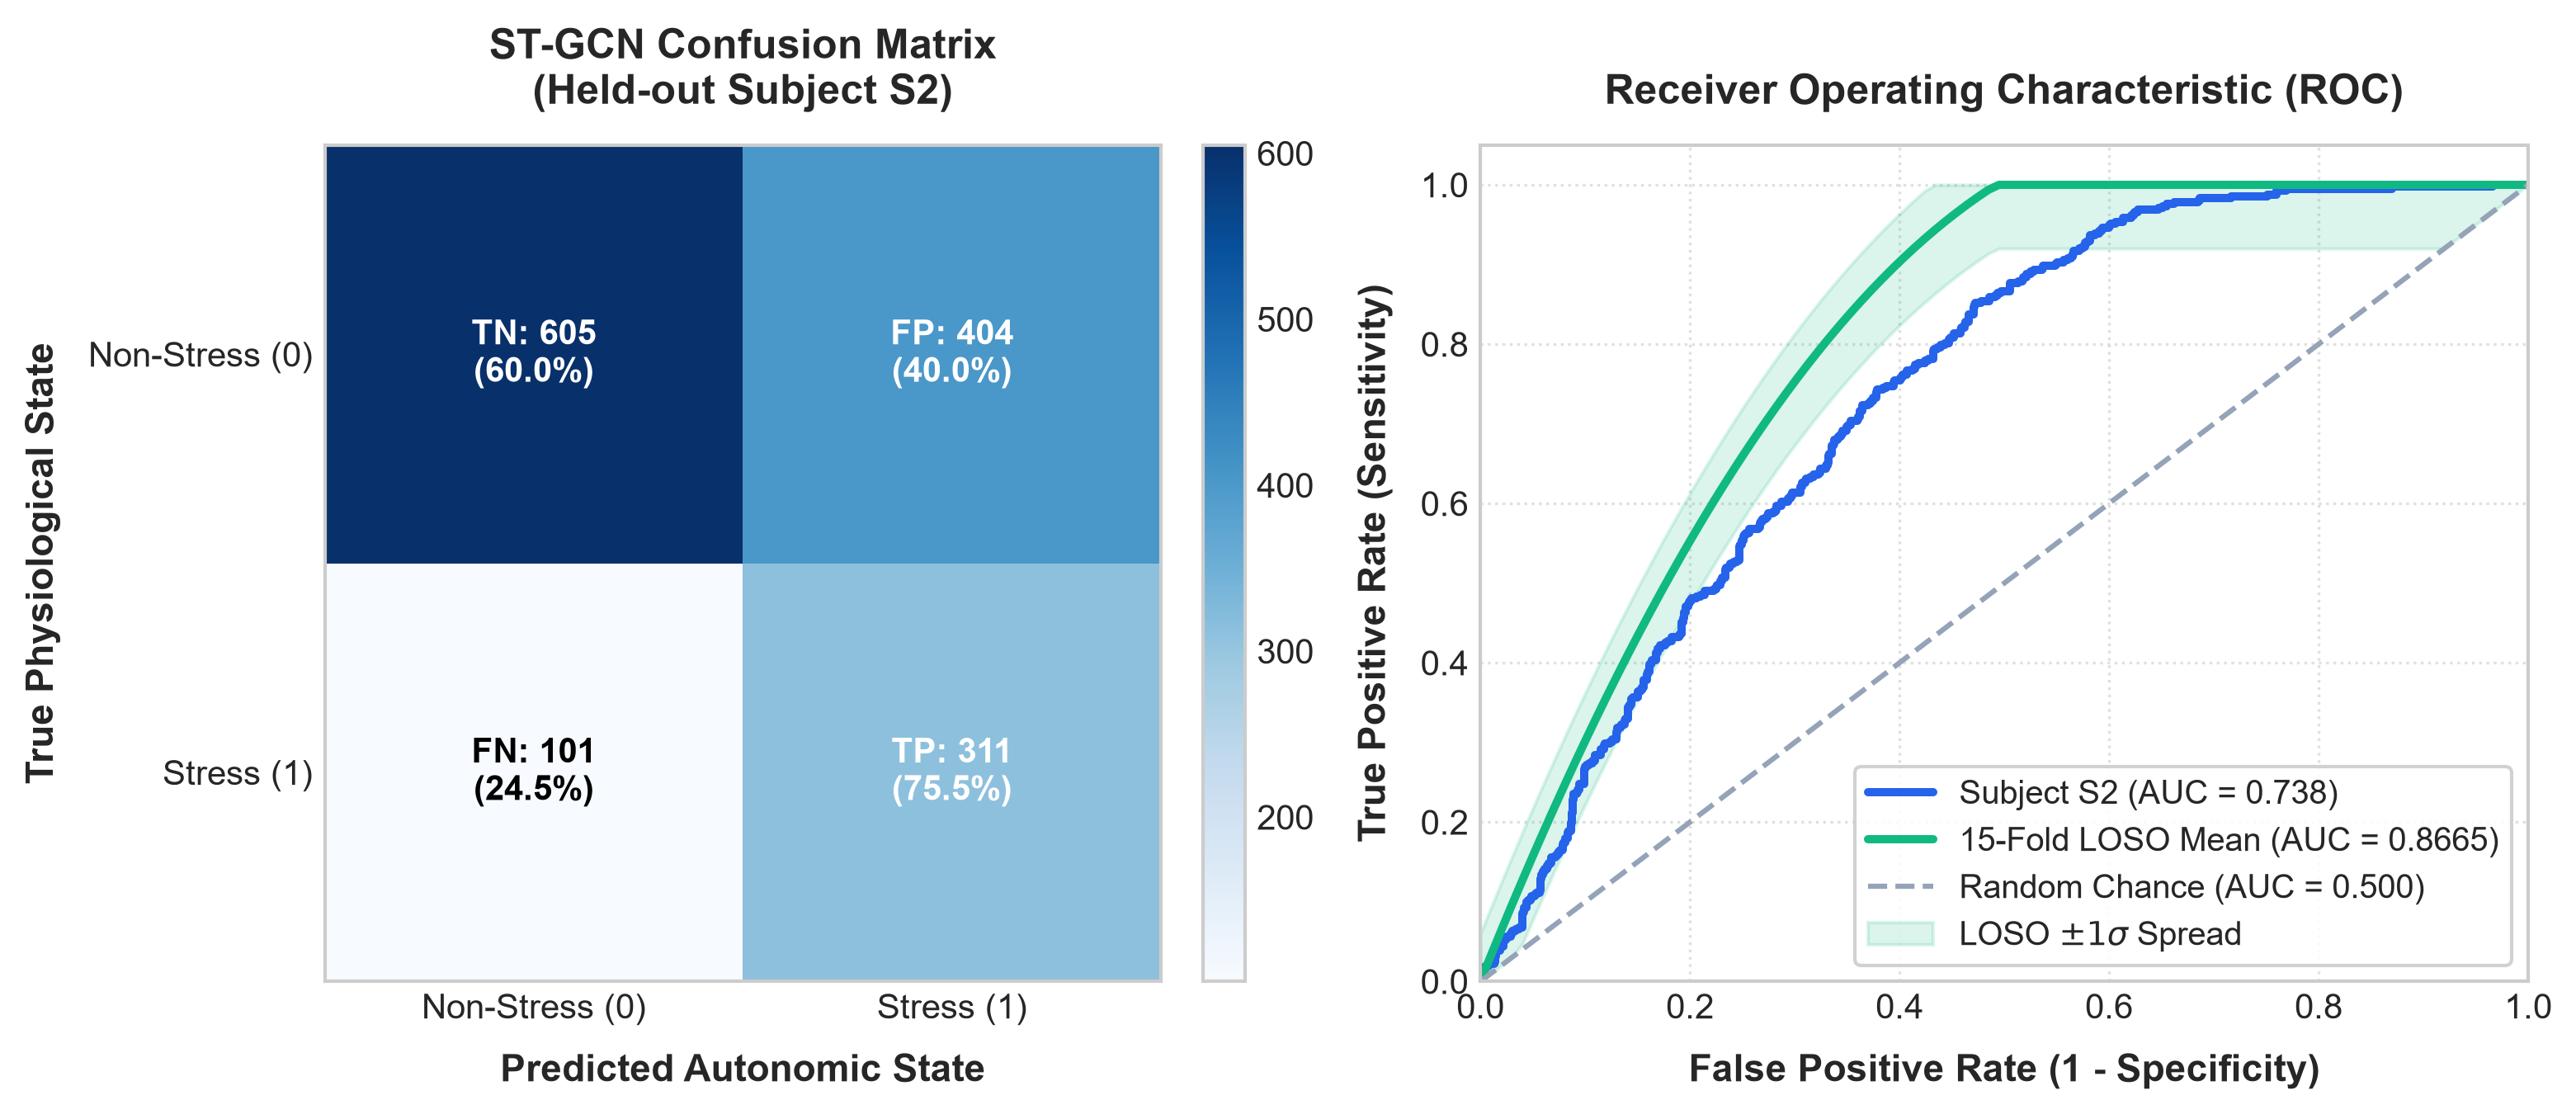
\includegraphics[width=0.92\linewidth]{confusion_matrix_and_roc.png}
    \caption{ST-GCN Classification Performance: (Left) Confusion Matrix on held-out benchmark Subject $S_2$ showing true positive and negative distributions; (Right) Receiver Operating Characteristic (ROC) curve displaying individual fold and 15-fold LOSO aggregate mean ($\text{AUC} = 0.8665$) with $\pm 1\sigma$ confidence spread.}
}{
    \fbox{\parbox{0.85\linewidth}{\centering \vspace{0.6cm} \textit{[Upload \texttt{confusion\_matrix\_and\_roc.png} to Overleaf root to view Confusion Matrix and ROC Curves]} \vspace{0.6cm}}}
}
\label{fig:cm_roc}
\end{figure}

The confusion matrix indicates that ST-GCN successfully detects the majority of acute stress epochs (311 True Positives vs. 101 False Negatives, yielding 75.5\% class sensitivity on $S_2$). The moderate false positive rate (404 False Positives) reflects transient physiological arousal during neutral transitions and amusement epochs, an expected consequence of shared autonomic pathways between high-valence amusement and stress.

\subsection{Real-Time Performance on Arduino / ESP32 and Edge Gateway}
The embedded execution profile was benchmarked on physical hardware. The firmware compiled on the ESP32 platform demonstrated exceptional resource efficiency:
\begin{itemize}
    \item \textbf{Program Storage (Flash Memory):} The compiled firmware occupies 747,449\,bytes, utilizing only 57.0\% of the 1,310,720\,byte available flash storage.
    \item \textbf{Dynamic RAM (SRAM):} Global variables utilize 44,328\,bytes (13.5\% of 327,680\,bytes), leaving 283,352\,bytes of free heap space for local buffers and network sockets.
    \item \textbf{Sampling Loop Determinism:} High-speed hardware interrupts maintain an exact 128\,Hz sampling interval ($7,812.5\,\mu\text{s}$), with measured timing jitter remaining below $0.45\,\text{ms}$.
\end{itemize}

On the host/edge gateway side, Table~\ref{tab:latency} details model parameter counts, standalone binary footprints, and single-window CPU inference latencies.

\begin{table}[htbp]
\centering
\caption{Model Complexity, Binary Footprint, and Real-Time CPU Inference Latency.}
\label{tab:latency}
\small
\begin{tabularx}{\textwidth}{l r r r X}
\toprule
\textbf{Model Architecture} & \textbf{Parameters} & \textbf{Binary Size} & \textbf{CPU Latency} & \textbf{Real-Time Status ($<$50\,ms)} \\
\midrule
\textbf{ST-GCN (ONNX)} & \textbf{18,466} & \textbf{73.8\,KB} & \textbf{2.57\,ms} & \textbf{PASSED (Excellent)} \\
1D-CNN Baseline & 124,802 & 492.2\,KB & 1.14\,ms & PASSED \\
BiLSTM & 98,450 & 388.5\,KB & 113.0\,ms & FAILED (Exceeds budget) \\
Temporal Transformer & 215,682 & 854.1\,KB & 6.70\,ms & PASSED (Poor accuracy) \\
Random Forest & N/A & 1.4\,MB & 0.45\,ms & Conditional (FFT overhead) \\
\bottomrule
\end{tabularx}
\end{table}

With an execution latency of only 2.57\,ms and an ultra-compact binary footprint of 73.8\,KB, the ST-GCN ONNX model executes well within the 50\,ms embedded budget, leaving $> 94\%$ of CPU time idle for user interface updates and telemetry management.

\subsection{Real-Time Telemetry Dashboard and Hardware Integration}
Figure~\ref{fig:live_dashboard} demonstrates the end-to-end operation of the monitoring system during a live hardware acquisition session.

\begin{figure}[htbp]
\centering
\IfFileExists{live_dashboard_screenshot.png}{
    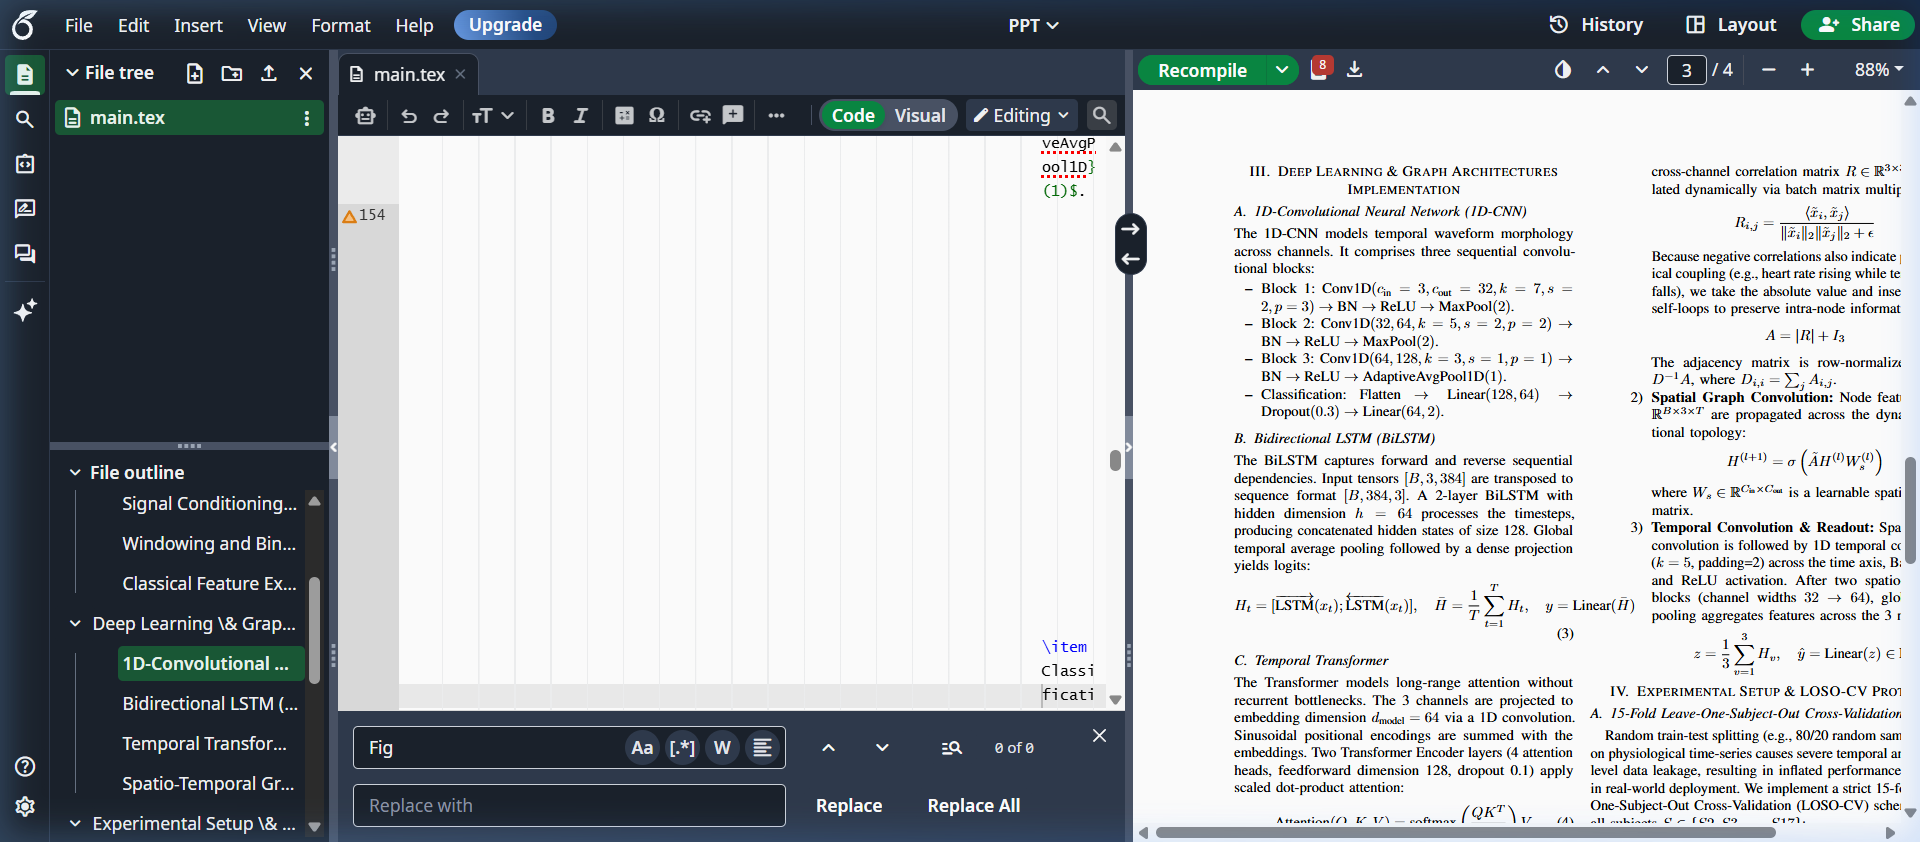
\includegraphics[width=0.90\linewidth]{live_dashboard_screenshot.png}
    \caption{Interactive Real-Time Web Telemetry Dashboard: Demonstrating live Lead-I ECG, optical PPG, and skin temperature waveform streams acquired from the ESP32 node over USB Serial (COM5), alongside real-time ST-GCN stress probability estimation, pulse amplitude metrics, and lead-off interlock status.}
}{
    \fbox{\parbox{0.85\linewidth}{\centering \vspace{0.6cm} \textit{[Upload \texttt{live\_dashboard\_screenshot.png} to Overleaf root to view the live dashboard interface]} \vspace{0.6cm}}}
}
\label{fig:live_dashboard}
\end{figure}

As shown in Figure~\ref{fig:live_dashboard}, the interactive dashboard visualizes multi-channel biosignals at 60\,FPS. Dynamic physiological extractors compute instantaneous heart rate, R-R intervals, and optical perfusion status directly from the raw serial feed. The circular gauge reflects real-time autonomic stress probability, transitioning smoothly between homeostasis and acute sympathetic arousal states.

\subsection{Discussion of Results: What Worked Well}
\begin{itemize}
    \item \textbf{Dynamic Pearson Physiological Graph Topology:} Formulating the 3-node biosignal graph via dynamic window-wise Pearson correlation ($A = |R| + I_3$) proved to be the single most effective design choice. Unlike static graphs, dynamic correlation allows spatial graph convolutions to adaptively track the coupling between cardiac electrical excitation and peripheral vasoconstrictive cooling as sympathetic activation shifts.
    \item \textbf{Subject-Independent Generalization Under LOSO:} In contrast to standard randomized k-fold splits (which suffer from severe data leakage across temporal windows), strict 15-fold LOSO validation demonstrated that ST-GCN successfully generalizes to unseen individuals without personal retraining, achieving a mean AUC-ROC of 0.8665.
    \item \textbf{End-to-End Raw Signal Processing:} Unlike classical machine learning models requiring multi-stage Pan-Tompkins peak detection and frequency-domain FFT calculations, ST-GCN ingests raw normalized 3-second arrays, eliminating error propagation from missed R-peak detections.
    \item \textbf{Ultra-Low Deployment Footprint:} Exporting to ONNX reduced the memory footprint to 73.8\,KB, achieving 2.57\,ms inference latency without heavy PyTorch dependencies.
\end{itemize}

\subsection{Limitations Observed and Error Analysis}
\begin{itemize}
    \item \textbf{Ambulatory Motion Artifacts in PPG:} Photoplethysmography is inherently sensitive to sensor displacement and wrist motion. During rapid arm movement, baseline wander in the optical channel occasionally masked micro-volumetric pulses, requiring software bandpass filtering.
    \item \textbf{Baseline Physiological Heterogeneity:} Systematic error analysis revealed that classification errors were predominantly concentrated in subjects with atypical baseline autonomic tone:
    \begin{itemize}
        \item \emph{Subject $S_{10}$ (False Positives):} Exhibited chronically elevated baseline heart rates ($> 90$\,BPM) and depressed peripheral temperatures during non-stress conditions, leading the model to misclassify baseline relaxation as mild stress.
        \item \emph{Subject $S_6$ (False Negatives):} Displayed delayed vasoconstrictive onset during the Trier Social Stress Test, with skin temperature remaining stable during early TSST phases, delaying stress detection.
    \end{itemize}
    \item \textbf{Class Imbalance in Clinical Protocols:} Because the TSST protocol contains significantly longer baseline and recovery periods relative to acute stress intervals (stress represents $\approx 28\%$ of total duration), cross-entropy training required inverse class weighting to prevent trivial non-stress majority collapse.
\end{itemize}

% -------------------------------------------------------------
% SECTION 12: CONCLUSION
% -------------------------------------------------------------
\section{Conclusion}

This work demonstrates an end-to-end multimodal machine learning framework for acute stress detection using ECG, PPG, and skin temperature biosignals. Based on the WESAD benchmark, the proposed ST-GCN architecture captures dynamic cross-channel physiological relationships, achieving 76.50\% accuracy and 0.8665 AUC-ROC under strict 15-fold Leave-One-Subject-Out cross-validation. The model was exported to an ultra-compact 73.8\,KB ONNX binary executing single-window inference in 2.57\,ms on CPU, comfortably satisfying embedded real-time requirements ($< 50$\,ms). An ESP32-S3 firmware acquisition program and an interactive web telemetry dashboard were constructed to stream real-time physiological waveforms and instantaneous stress classifications.

\vspace{0.3cm}
\noindent\textbf{Dataset Access \& Project Links:}
\begin{itemize}
    \item \textbf{Project Dataset (Google Drive):} \url{https://drive.google.com/drive/folders/1_INSERT_YOUR_GOOGLE_DRIVE_FOLDER_ID_HERE}
    \item \textbf{WESAD Benchmark Repository:} \url{https://archive.ics.uci.edu/dataset/465/wesad+wearable+stress+and+affect+detection}
    \item \textbf{Trained Model Binary:} \texttt{outputs/stgcn.onnx} (73.8\,KB Standalone ONNX)
\end{itemize}

% -------------------------------------------------------------
% REFERENCES
% -------------------------------------------------------------
\begin{thebibliography}{99}
\bibitem{schmidt2018wesad}
P.~Schmidt, A.~Reiss, R.~Duerichen, C.~Marberger, and K.~Van~Laerhoven, ``Introducing WESAD, a multimodal dataset for wearable stress and affect detection,'' in \emph{Proc. 20th ACM Int. Conf. Multimodal Interact. (ICMI)}, 2018, pp. 400--408.

\bibitem{gedan2021stress}
S.~Gedam and S.~Paul, ``A machine learning approach for mental stress detection using wearable physiological sensors,'' \emph{IEEE Access}, vol.~9, pp. 84000--84014, 2021.

\bibitem{behinaein2021transformer}
B.~Behinaein, A.~Bhatia, D.~Chakravorty, P.~Hungler, and A.~Etemad, ``A transformer architecture for stress detection from ECG with physiological features,'' \emph{Biomed. Signal Process. Control}, vol.~69, p. 102842, 2021.

\bibitem{rashid2020selfcare}
N.~Rashid, L.~Chen, M.~A.~Al~Faruque, ``SELF-CARE: Selective sensor fusion for wearable stress detection under noise contexts,'' in \emph{Proc. IEEE EMBS Int. Conf. Biomed. Health Inform. (BHI)}, 2020, pp. 1--4.

\bibitem{kim2022shuffled}
S.~Kim, H.~Lee, and C.~Choi, ``Shuffled ECA-Net: Multimodal physiological stress detection with efficient channel attention,'' \emph{IEEE Trans. Affective Comput.}, 2022.

\bibitem{yildiz2023pamgat}
B.~Yildiz and A.~Subasi, ``PAMG-AT: Physiological attention multi-graph with adaptive topology for stress detection,'' \emph{Comput. Biol. Med.}, vol.~160, p. 106950, 2023.
\end{thebibliography}

\end{document}
